\documentclass[10pt,journal]{IEEEtran}
\usepackage{fontspec,xeCJK}
\setmainfont{Times New Roman}
\setsansfont{Arial}
\setmonofont{Consolas}
\setCJKmainfont{SimSun}[BoldFont=SimHei,ItalicFont=KaiTi,BoldItalicFont=SimHei]
\usepackage{amsmath,amssymb,graphicx,booktabs,array,xcolor,placeins,stfloats,url}
\usepackage[hidelinks]{hyperref}
\definecolor{loss}{HTML}{B6574E}
\definecolor{gain}{HTML}{307F76}
\renewcommand{\abstractname}{摘要}
\renewcommand{\IEEEkeywordsname}{关键词}
\renewcommand{\tablename}{表}
\renewcommand{\figurename}{图}
\renewcommand{\arraystretch}{1.15}
\setlength{\tabcolsep}{4pt}
\setlength{\textfloatsep}{10pt plus 2pt minus 1pt}
\setlength{\dbltextfloatsep}{10pt plus 2pt minus 1pt}
\setlength{\floatsep}{8pt plus 2pt minus 1pt}
\renewcommand{\topfraction}{.95}
\renewcommand{\dbltopfraction}{.95}
\renewcommand{\textfraction}{.04}
\renewcommand{\floatpagefraction}{.8}
\renewcommand{\dblfloatpagefraction}{.8}
\setcounter{topnumber}{5}
\setcounter{dbltopnumber}{5}
\setcounter{totalnumber}{10}
\makeatletter
\setlength{\@fptop}{0pt}
\setlength{\@fpsep}{14pt}
\setlength{\@fpbot}{0pt plus 1fil}
\setlength{\@dblfptop}{0pt}
\setlength{\@dblfpsep}{14pt}
\setlength{\@dblfpbot}{0pt plus 1fil}
\makeatother
\clubpenalty=10000\widowpenalty=10000
\begin{document}
\title{PAMF网络分支消融：跨日跨接收机泛化}

\author{仅分类损失的监督训练\quad 实验结果报告\quad 2026年10月26日}

\maketitle

\begin{abstract}
本报告呈现PAMF直接识别在跨日跨接收机群体上的五项网络分支消融，并增加跨接收机126000包与跨日跨接收机42000包两类互斥群体的综合统计。每组含三个模型种子。综合指标先按种子和场景合并168000条样本对应的混淆矩阵，再计算准确率与宏平均F1；相对变化为“变体减完整网络”，负值表示下降。分群与综合结果均保留种子离散度和反向结果。
\end{abstract}

\begin{IEEEkeywords}射频指纹识别，PAMF，结构消融，跨日跨接收机泛化。\end{IEEEkeywords}

\section{实验设置与统计口径}

本报告主分析采用日期与接收机同时未见的测试群体，并补充两类互斥测试群体的综合统计；全部结果均为PAMF直接识别。标准六类划分中，训练使用源接收机的三天数据，测试使用7个目标接收机在另一较早日期的观测；每景42000包。该日期早于训练日期，不解释为未来日期外推。

识别器采用仅分类损失的监督控制配方，保留原输入与信道增强设置，既有默认分类头联合训练。完整网络与五个结构变体均使用相同划分和50轮预算，每组3个独立模型种子，共18个已完成模型。本文没有新增训练、预测或目标真值访问。

每个模型的全部声明场景决策冻结后，由独立CPU完成评分。六景均值不含clean，先在每个种子内对六个信道场景等权平均，再报告三个种子的均值与样本标准差。宏平均F1按全部六类计算。所有指定变体、三个种子和七个场景均保留。

\section{结构控制与差值定义}

\noindent\textbf{去除显式时间坐标}。保留路径描述及共享骨干，只去除描述中的显式时间坐标；不是删除时域骨干。\par

\noindent\textbf{去除路径描述支路}。完整移除SIG-TIME路径描述分支；基础时频表示继续训练。这就是“去SIG-TIME”，不能重复计为另一组。\par

\noindent\textbf{去除功放相关支路}。移除功放相关计算和统计投影，其他结构继续按同预算训练。\par

\noindent\textbf{去除参考响应支路}。移除公共参考响应及其投影，保留其他身份表示。\par

\noindent\textbf{打乱参考模板相位}。固定扰乱公共模板频谱相位并保留幅度谱；训练与测试使用同一模板。\par

相对变化统一定义为变体减完整PAMF，同种子相减后再统计。负值表示性能下降，正值表示性能提高；\ensuremath{\pm}表示三个配对差的样本标准差，不是置信区间，也不是两组标准差相加。暖红与青绿分别标记下降和提高，图中同时使用正负号与点形，避免只依赖颜色。

\begin{equation}\Delta_{s}=M_{s,\mathrm{variant}}-M_{s,\mathrm{full}},\quad \bar\Delta=\frac{1}{3}\sum_{s=1}^{3}\Delta_s.\end{equation}

\begin{table*}[!t]

\caption{PAMF直接识别：跨日跨接收机测试结果（\%，三种子均值\ensuremath{\pm}样本标准差）。}

\label{tab:absolute}

\centering\small

\begin{tabular*}{\textwidth}{@{\extracolsep{\fill}}lrrrr@{}}

\toprule

网络结构 & \multicolumn{2}{c}{clean} & \multicolumn{2}{c}{六景均值} \\

\cmidrule(lr){2-3}\cmidrule(lr){4-5}

 & 准确率 & 宏平均F1 & 准确率 & 宏平均F1 \\

\midrule

完整 PAMF & \textbf{79.59\ensuremath{\pm}2.46} & \textbf{78.88\ensuremath{\pm}2.51} & \textbf{69.44\ensuremath{\pm}0.66} & \textbf{69.07\ensuremath{\pm}0.69} \\

去除显式时间坐标 & 79.14\ensuremath{\pm}2.13 & 78.33\ensuremath{\pm}2.22 & 68.91\ensuremath{\pm}0.51 & 68.49\ensuremath{\pm}0.46 \\

去除路径描述支路 & 80.81\ensuremath{\pm}1.20 & 80.40\ensuremath{\pm}1.23 & 70.29\ensuremath{\pm}0.44 & 70.00\ensuremath{\pm}0.48 \\

去除功放相关支路 & 77.97\ensuremath{\pm}1.16 & 77.15\ensuremath{\pm}1.02 & 63.81\ensuremath{\pm}2.20 & 63.01\ensuremath{\pm}2.41 \\

去除参考响应支路 & 79.05\ensuremath{\pm}1.45 & 78.33\ensuremath{\pm}1.46 & 69.14\ensuremath{\pm}0.60 & 68.79\ensuremath{\pm}0.60 \\

打乱参考模板相位 & 78.52\ensuremath{\pm}2.14 & 77.78\ensuremath{\pm}2.17 & 69.48\ensuremath{\pm}0.58 & 69.13\ensuremath{\pm}0.64 \\

\bottomrule

\end{tabular*}

\end{table*}

\begin{table*}[!t]

\caption{同种子相对变化：结构变体减完整PAMF（百分点）。负值为下降，正值为提高；\ensuremath{\pm}为配对差的样本标准差。}

\label{tab:paired}

\centering\small

\begin{tabular*}{\textwidth}{@{\extracolsep{\fill}}lrrrr@{}}

\toprule

网络结构 & \multicolumn{2}{c}{clean} & \multicolumn{2}{c}{六景均值} \\

\cmidrule(lr){2-3}\cmidrule(lr){4-5}

 & 准确率 & 宏平均F1 & 准确率 & 宏平均F1 \\

\midrule

去除显式时间坐标 & \textcolor{loss}{-0.45\ensuremath{\pm}1.98} & \textcolor{loss}{-0.55\ensuremath{\pm}2.22} & \textcolor{loss}{-0.54\ensuremath{\pm}1.04} & \textcolor{loss}{-0.58\ensuremath{\pm}1.08} \\

去除路径描述支路 & \textcolor{gain}{+1.22\ensuremath{\pm}2.36} & \textcolor{gain}{+1.53\ensuremath{\pm}2.50} & \textcolor{gain}{+0.85\ensuremath{\pm}0.25} & \textcolor{gain}{+0.94\ensuremath{\pm}0.29} \\

去除功放相关支路 & \textcolor{loss}{-1.62\ensuremath{\pm}2.40} & \textcolor{loss}{-1.73\ensuremath{\pm}2.38} & \textcolor{loss}{-5.63\ensuremath{\pm}1.95} & \textcolor{loss}{-6.06\ensuremath{\pm}2.06} \\

去除参考响应支路 & \textcolor{loss}{-0.54\ensuremath{\pm}1.02} & \textcolor{loss}{-0.55\ensuremath{\pm}1.05} & \textcolor{loss}{-0.30\ensuremath{\pm}0.06} & \textcolor{loss}{-0.28\ensuremath{\pm}0.12} \\

打乱参考模板相位 & \textcolor{loss}{-1.07\ensuremath{\pm}0.40} & \textcolor{loss}{-1.09\ensuremath{\pm}0.44} & \textcolor{gain}{+0.04\ensuremath{\pm}0.23} & \textcolor{gain}{+0.06\ensuremath{\pm}0.27} \\

\bottomrule

\end{tabular*}

\end{table*}

\section{结果与讨论}

表~\ref{tab:absolute}~给出绝对指标，表~\ref{tab:paired}~和图~\ref{fig:paired_changes}~给出同种子配对变化。

去除功放相关支路的六景准确率变化为-5.63\ensuremath{\pm}1.95个百分点，宏平均F1变化为-6.06\ensuremath{\pm}2.06个百分点。三个种子的六景准确率变化均为负，说明这一结构在当前监督配方与双重变化群体中有较一致的作用。clean变化的种子方向仍不完全一致，不能声称所有条件都同等受益。

去除路径描述支路的六景准确率变化为+0.85\ensuremath{\pm}0.25个百分点，三个种子方向均为正；clean变化为+1.22\ensuremath{\pm}2.36个百分点。该结果不支持在本测试群体中声称完整SIG-TIME支路必然提高识别性能，也不能由此直接改变其他训练配方的结构。

去除参考响应支路的六景变化为-0.30\ensuremath{\pm}0.06个百分点，三个种子均为负。打乱参考模板相位在clean下变化为-1.07\ensuremath{\pm}0.40个百分点，但六景变化为+0.04\ensuremath{\pm}0.23个百分点，接近零。参考支路收益与“真实模板相位必不可少”不是同一个命题。

去除显式时间坐标的六景变化为-0.54\ensuremath{\pm}1.04个百分点，两个种子下降、一个提高。该控制保留路径描述和骨干中的时域信息，不能把结果解释成移除了整个时间建模能力。

\begin{figure*}[!t]

\centering

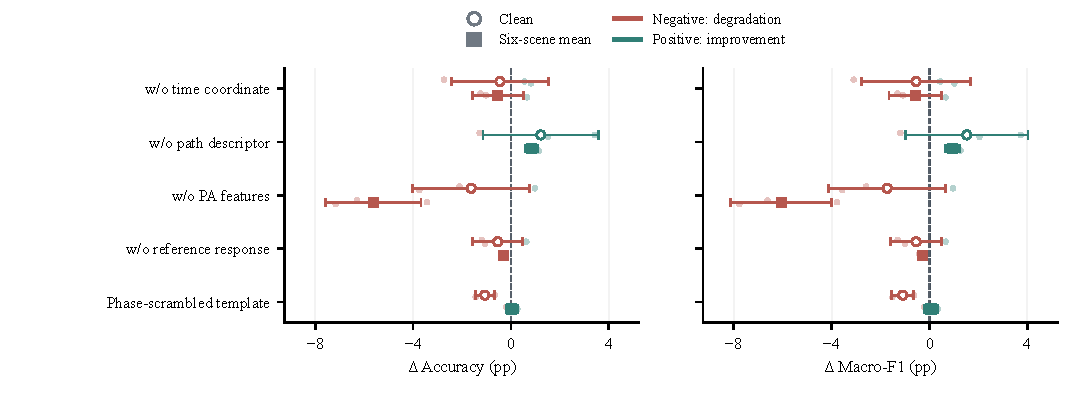
\includegraphics[width=\textwidth]{../figures/paired_changes.pdf}

\caption{同种子配对差：变体减完整PAMF。误差线为3个配对差的样本标准差，浅色小点为每个种子的配对差；负值表示下降，正值表示提高。}

\label{fig:paired_changes}

\end{figure*}

\begin{figure*}[!t]

\centering

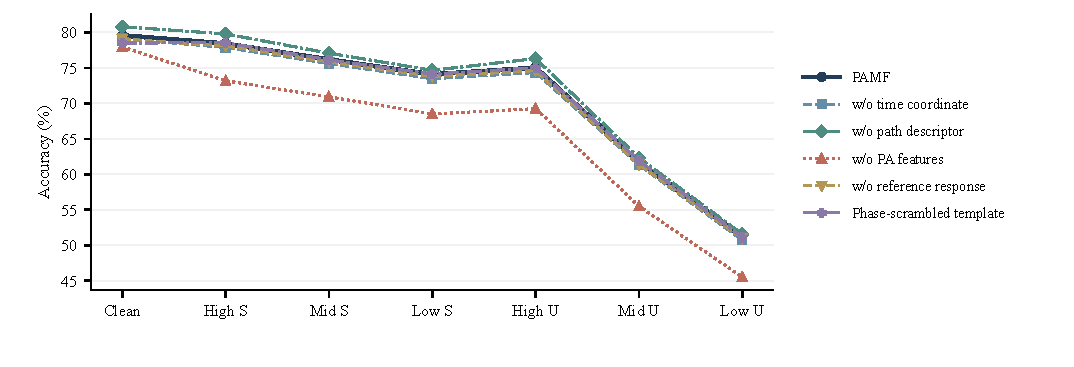
\includegraphics[width=\textwidth]{../figures/seven_scene_accuracy.pdf}

\caption{跨日跨接收机、PAMF直接识别的逐场景准确率。每点为3个训练种子均值。S为郊区，U为城市；不同线型和点形便于黑白打印。}

\label{fig:seven_scene_accuracy}

\end{figure*}

\begin{figure*}[!t]

\centering

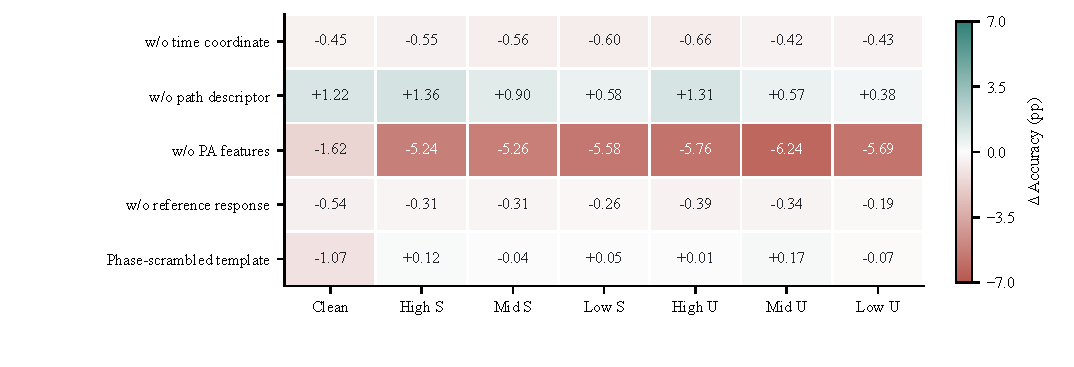
\includegraphics[width=\textwidth]{../figures/scene_changes.pdf}

\caption{逐场景配对准确率变化，单位为百分点。暖红表示变体低于完整PAMF，青绿表示变体高于完整PAMF；色标以0为中心且对称。}

\label{fig:scene_changes}

\end{figure*}

图~\ref{fig:seven_scene_accuracy}~与图~\ref{fig:scene_changes}~按七个固定场景呈现结果。整体均值与逐场景结论并不等价，单个场景的正向或负向变化均应保留。

\section{两类测试的综合统计}

综合测试仅合并两类互斥群体：跨接收机126000包、跨日跨接收机42000包，每个场景共168000包。准确率按实际样本合并计算，两类权重分别为75\%和25\%；不是两个准确率的简单平均。宏平均F1先合并两类六分类混淆矩阵，再按六类重算，不能直接加权或平均已有F1。

合并在每个模型种子、每个场景内独立完成。随后对六个信道场景等权平均，最后对三个模型种子计算均值与样本标准差；相对变化仍先按种子计算“变体减完整PAMF”。同一18个模型同时支持分群与综合统计，不增加模型重复数。

\begin{equation}C_{s,v}^{\mathrm{all}}=\sum_{g=1}^{2}C_{s,v}^{(g)},\quad N=168000.\end{equation}

\begin{equation}\operatorname{MacroF1}(C)=\frac{1}{6}\sum_{k=1}^{6}\frac{2C_{kk}}{\sum_j C_{kj}+\sum_i C_{ik}}.\end{equation}

完整PAMF的综合clean准确率为82.67\ensuremath{\pm}1.26\%，综合六景准确率为70.91\ensuremath{\pm}0.46\%，综合六景宏平均F1为70.65\ensuremath{\pm}0.41\%。去除功放相关支路的综合六景准确率变化为-6.82\ensuremath{\pm}1.01个百分点；去除路径描述支路的变化为-0.45\ensuremath{\pm}0.61个百分点。后者与跨日跨接收机分群中的+0.85\ensuremath{\pm}0.25个百分点方向不同，说明分群与综合结论应分别保留。

综合结果反映既有样本分布，跨接收机群体占75\%，对综合值影响较大；它不能代替各群体结果。综合样本全部来自目标接收机，日期包含训练中已见日期和另一较早未见日期。所有综合结果均来自既有冻结混淆矩阵，未新增预测、真值访问或模型训练。

表~\ref{tab:pooled}~和图~\ref{fig:composite_testing}~给出综合结果。

\begin{table*}[!t]

\caption{两类测试合并统计（\%，每景168000包，三种子均值±样本标准差）。宏平均F1由合并混淆矩阵重算。}

\label{tab:pooled}

\centering\small

\begin{tabular*}{\textwidth}{@{\extracolsep{\fill}}lrrrr@{}}

\toprule

网络结构 & \multicolumn{2}{c}{综合clean} & \multicolumn{2}{c}{综合六景均值} \\

\cmidrule(lr){2-3}\cmidrule(lr){4-5}

 & 准确率 & 宏平均F1 & 准确率 & 宏平均F1 \\

\midrule

完整 PAMF & \textbf{82.67\ensuremath{\pm}1.26} & \textbf{82.24\ensuremath{\pm}1.28} & \textbf{70.91\ensuremath{\pm}0.46} & \textbf{70.65\ensuremath{\pm}0.41} \\

去除显式时间坐标 & 82.49\ensuremath{\pm}1.49 & 82.03\ensuremath{\pm}1.61 & 70.36\ensuremath{\pm}0.52 & 70.06\ensuremath{\pm}0.63 \\

去除路径描述支路 & 82.72\ensuremath{\pm}1.23 & 82.33\ensuremath{\pm}1.33 & 70.46\ensuremath{\pm}0.37 & 70.19\ensuremath{\pm}0.39 \\

去除功放相关支路 & 78.55\ensuremath{\pm}0.20 & 77.89\ensuremath{\pm}0.17 & 64.09\ensuremath{\pm}1.08 & 63.66\ensuremath{\pm}1.10 \\

去除参考响应支路 & 81.63\ensuremath{\pm}0.97 & 81.20\ensuremath{\pm}0.97 & 70.40\ensuremath{\pm}0.45 & 70.14\ensuremath{\pm}0.34 \\

打乱参考模板相位 & 81.92\ensuremath{\pm}0.95 & 81.46\ensuremath{\pm}0.96 & 70.67\ensuremath{\pm}0.42 & 70.43\ensuremath{\pm}0.32 \\

\bottomrule

\end{tabular*}

\end{table*}

\begin{figure*}[!t]

\centering

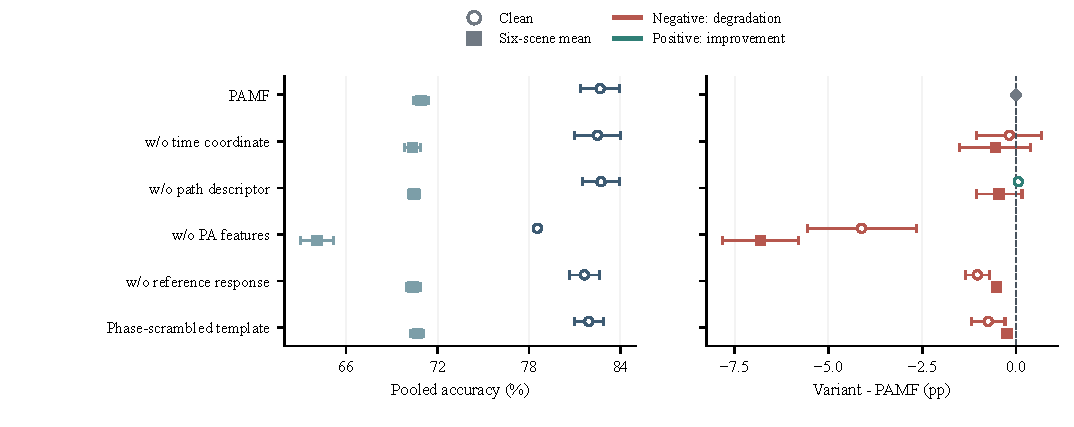
\includegraphics[width=\textwidth]{../figures/composite_testing.pdf}

\caption{两类互斥测试综合：每景合并168000条样本。左为综合准确率，右为同种子“变体减完整PAMF”；完整模型记作0参考。每点为3个训练种子均值；误差线左为指标标准差，右为配对差标准差。clean与六景均值分列。}

\label{fig:composite_testing}

\end{figure*}

\section{结论与适用边界}

本报告按用户指定范围事后筛选展示项，未依据成绩删除种子、重排训练或选择性重跑。结论只适用于当前六类划分、监督分类目标、已列出的分群结果和既有样本权重下的综合测试；不能外推到其他训练目标。三个种子不足以支撑普遍显著性结论；单支路改动的条件差异也不是可相加的独立因果贡献。

\noindent\textbf{结论。} 当前监督控制中，功放相关支路的六景作用最明显；参考响应支路有较小且同种子方向一致的六景作用。完整路径描述和显式时间坐标的收益不能预设为普遍成立。原始指标、三个配对差及可编辑矢量图随本报告导出，便于论文使用与独立复算。

\FloatBarrier

\end{document}
